%% ----------------------------------------------------------------
%% PreviousWork.tex
%% ---------------------------------------------------------------- 
\chapter{Previous Work} 
\label{Chapter:Previous Work}
\chapterpreamble{To avoid duplicating work done by other parties an investigation into the current standing of related fields was undertaken, both in academia and the education industry. This showed where improvements could be made and identified methods and tools that could be used within the project. The areas studied were: types of assessment, eAssessment, quiz standards, video accessibility and usability, and analysis of video usage.}

A \gls{MLE} is the overall system used by an educational establishment to facilitate and manage learning. This will be comprised of several subsystems (as seen in \autoref{Figure: MLE}).

\begin{figure}[h]
	\centering 
		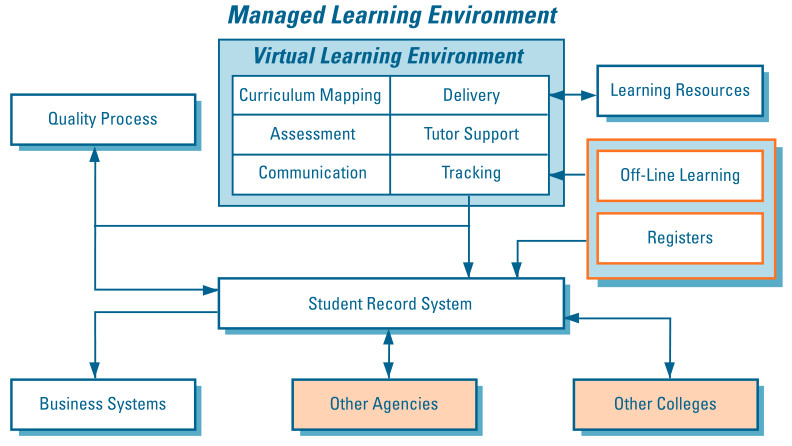
\includegraphics[scale=0.4]{../figures/MLE.png} 		
	\caption{\label{Figure: MLE} Components of an \gls{MLE} \citep{mle}} 	
\end{figure}

This project focuses on the assessment system in the \gls{VLE}.

\section{Types of Assessment}
\label{Section: Types of Assessment}

In education, summative (or `assessment of learning' \citep{digiassess}) and formative (or `assessment for learning' \citep{digiassess}) assessments are often used to provide different types of feedback to students and show their level of progression and competence. The method of assessment will depend on the perspective of the assessor (see \autoref{Table: Perspectives on Learning}).

Summative assessment is used when achievement levels need to be reported against a set of published criteria, often as an end of course evaluation. As all students are evaluated against the same criteria their results can be combined to form league tables etc. \citep{assessmentTypes}. These assessments are generally high-stakes so ``those being assessed are likely to do all they can to conceal ignorance and suggest competence" \citep{knight2001briefing}. The feedback from such assessments is usually a mark, often given as a level of achievement or competence rather than specific details on how the assessment could have been completed more successfully.

\begin{longtable}{|L{0.188}|L{0.248}|L{0.204}|L{0.25}|}
\caption[Perspectives on learning]{\label{Table: Perspectives on Learning} Perspectives on learning and approaches to assessment and feedback (from \citep{digiassess})} \\
\hline \textbf{Perspective on learning} & \textbf{Assumption} & \textbf{Assessment} & \textbf{Feedback} \\ \hhline{|=|=|=|=|} \endhead
\multicolumn{4}{c}{Continues on the next page...} \endfoot
\endlastfoot
\textbf{Associative} & \textbf{Learning as acquiring competence} \newline Learners acquire knowledge by building associations between different concepts. \newline Learners gain skills by building progressively complex actions from component skills. & Concepts and competencies frequently assessed at micro level and in combination through macro-level tasks. & - Expert feedback focusing on weaknesses in skills and conceptual understanding \newline - Interactive environments for knowledge and skills acquisition \eoline
\textbf{Constructivist} & \textbf{Learning as achieving understanding} \newline Learners actively construct ideas by building and testing hypotheses. & Assessment by means of experimentation, discovery and inquiry-based tasks. & - Self-generated feedback arising from reflection and self-assessment \newline -Interactive discovery environments with opportunities for self-testing \eoline
\textbf{Social constructivist} & \textbf{Learning as achieving understanding} \newline Learners actively construct new ideas through collaborative activities and dialogue. & Collaborative and cooperative tasks involving shared expression of ideas. \newline Participation by learners in the design of assessment tasks. & - Peer feedback arising from collaborative activities and dialogue \newline -Interactive environments that support sharing and peer feedback \eoline
\textbf{Situative} & \textbf{Learning as social practice} \newline Learners develop their identities through participation in specific communities of practice. & Holistic assessment in authentic or simulated professional contexts. \newline Participation in social practices of inquiry and assessment. & - Socially produced feedback from multiple sources \newline - Feedback derived from authentic real-life tasks \newline - Interactive environments that simulate professional practice \eoline
\end{longtable}

Formative assessment is not strictly based on criteria but takes into account students' progress and effort \citep{assessmentTypes}. The marks given for formative assessments may use the performance of students from several occurrences. These performances may be inconsistent but these differences in behaviour can be used as a diagnostic to locate where problems are \citep{assessmentTypes}. Formative assessment must be student centred as its two main aims are to get students to recognise the gap between the understanding level they have achieved and what is required, and for the students to take action to close this gap \citep{usesOfAssessment}. To identify the gap immediate feedback on how to improve is required \citep{eps265979} and the disclosure of concepts that are difficult needs to be encouraged \citep{knight2001briefing} to be able to provide effective feedback. 

The choice to use formative or summative assessment will depend on the purpose of the test. If a level of competence is required then summative assessment would be more appropriate. However a test to highlight the areas that the students are struggling with would be better as a formative assessment.

\section{eAssessment}
An \gls{eAssessment} (also known as \gls{CAidA}, \gls{CAssA}, \gls{CBA}) is the process of making, viewing and scoring assessments using a computer. In this report these processes will be carried out by several tools - the ``\gls{authoring}" will be responsible for creating the questions and assembling the test and the ``\gls{delivery}" will be responsible for displaying and scoring the assessments. These tools must be interoperable, meaning they must use data formats that are compatible with each other.

This project focuses on the use of quizzes and polls within videos as a means of assessment.

\subsection{Quiz Definition Standards}
\label{Subsection:Quiz Definition Standards}
In order to store and display the questions in an \gls{eAssessment}, a schema for the questions must be defined. The only formally defined standard found was IMS Global's \gls{QTI} specification\footnote{\url{http://www.imsglobal.org/question/\#version2.1} (Accessed: 24 Nov 14)}. Some other quiz (wiki-like) definitions were found including Moodle's General Import Format Technology (GIFT)\footnote{\url{https://docs.moodle.org/28/en/GIFT_format} (Accessed: 24 Nov 14)} and Aiken formats\footnote{\url{https://docs.moodle.org/23/en/Aiken_format} (Accessed: 24 Nov 14)}.

GIFT is a question mark up by Moodle\footnote{\url{https://moodle.org} (Accessed: 24 Nov 14)} and allows the use of a text editor to create questions in some simple formats. There is a strict compliance to specific syntax required and for complex questions it is no longer intuitive \citep{failQTI}. Aiken is another mark up that is designed to be more easily human-readable, again it has strict syntax that must be adhered to or the imports to Moodle would fail.

\gls{QTI} is an industrial interoperability standard for \glspl{eAssessment}. The specification overview \citep{qtiOverview} splits the \gls{eAssessment} system into five systems: authoring tool, item bank, test construction tool, assessment delivery system and learning system (see \autoref{Figure: QTI components}).

\begin{figure}[h]
	\centering 
		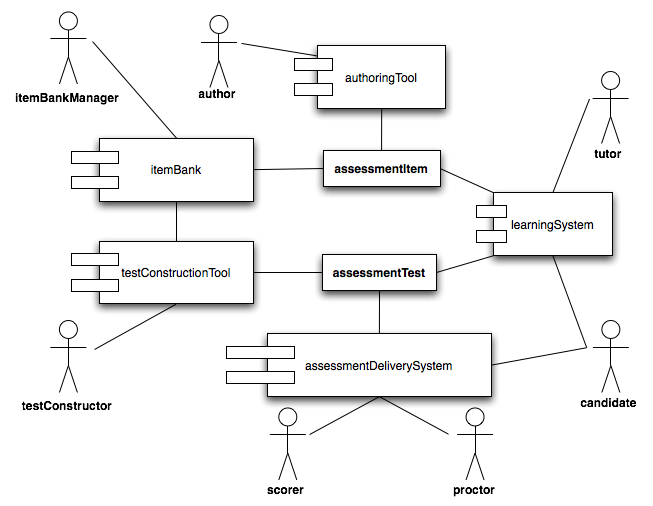
\includegraphics[scale=0.6]{../figures/componentsQTI.png} 		
	\caption{\label{Figure: QTI components} QTI components diagram \citep{qtiOverview}} 	
\end{figure}

In the \gls{QTI} definition the authoring tool is used to create individual questions. However many systems combine this with the Item Bank and Test Construction Tool. For this report ``\gls{authoring}" refers to this combination and, as such, an authoring tool is used to create whole quizzes.

In an academic review \Citeauthor{wikieassessment} (\citeyear{wikieassessment})~\citep{wikieassessment} state:
\begin{quote}
The major promise of QTI is that by introduction of common format developers can concentrate on developing innovative tools, whereas teachers can focus on defining new and groundbreaking methods of how to apply those tools in an online environment.
\end{quote}

It is a very complex specification with many ambiguous or optional elements. The complexity of the specification increases the likelihood for errors in the implementation as it opens up opportunities for developers to interpret the specification in different ways \citep{failQTI}. This means the intent of the original author may be lost.

\gls{QTI} v2.1 was finalised in 2012 \citep{qtiOverview} but up to this point the standard was not widely used \citep{eps265979} as there were several fundamental flaws in the standard. When the v2.1 draft was withdrawn in 2009 Rib Abel (IMS GLC CEO) was quoted as saying (on v2.0) ``it’s deficiencies are well known and IMS does not recommend implementation of it [\dots] the only version of QTI that is fully endorsed by IMS GLC is v1.2.1"\footnote{\url{http://lists.ucles.org.uk/public/ims-qti/2009-March/001463.html} (Accessed: 25 Nov 14)}. This standard gave definitions in natural language. These could often be long-winded and ambiguous, making the standard difficult to implement \citep{failQTI, Sclater2007}.

\gls{QTI} v2.1 defines 18 types of interaction (question, answers and response patterns) \citep{qtiImplementation}:
\begin{multicols}{3}
\begin{enumerate}
\item Choice
\item Order
\item Associate
\item Match
\item Gap match
\item Inline choice
\item Text entry
\item Extended text
\item Hot text
\item Hotspot
\item Select point
\item Graphic order
\item Graphic associate
\item Graphic gap match
\item Position object
\item Slider
\item Drawing
\item Upload file
\end{enumerate}
\end{multicols}

In addition, assessment items can have template and/or adaptive behaviour giving 72 options for each item's type. 

Template items have variables in the questions and answers. These are set as the question is viewed. This allows similar questions to be defined using the same assessment item (e.g. changing the numbers in a maths problem).

Adaptive items are scored over a series of questions. Different questions are displayed based on the answer given for the previous question(s) in the sequence. This branching behaviour is defined by setting the \lstinline!adaptive! attribute to \lstinline!true!. 

\subsection{Usage of Video in eAssessment}
\label{Subsection:Usage of Video in eAssessment}
Video is often used as a medium to convey educational material as it appeals to different learning styles. Academics found that when video is streamed there is a lack of interactivity and user control \citep{eps267281, DeBoer}. To involve the user more, interactive elements must be added. \Citeauthor{eps267281} \citep{eps267281} found that 75\% of users agreed or strongly agreed that interactive video had enhanced their learning experience but at the time of the paper (\citeyear{eps267281}) they could find no evidence of interactive video being used as a learning tool. There are now some interactive videos being used as a learning tool \citep{nadia} but not widely in \glspl{MLE}.

Interactive videos have often been implemented in Flash \citep{interactiveVideo, eps267281}. This is no longer supported on many devices in favour of HTML5 technologies \citep{flashDead}. The interactivity in HTML5 video players is generally implemented using clickable areas or pop ups \citep{interactiveHTML5}. HTML5 video players do not require an external plug-in to run so will be browser independent \citep{epifania2011design, interactiveHTML5} however some standards are not implemented in all browsers. 

Interactive videos including polls and quizzes is one method that could be used to give a formative assessment. This would give immediate, meaningful feedback, a key feature of formative assessment \citep{eps265979}. Having the questions integrated into the video allows the appropriate sections to be automatically re-watched, encouraging immediate action on feedback. 

\subsection{Accessibility and Usability}
\label{Subsection:Accessibility and Usability}
To allow interoperability between the \gls{eAssessment} systems the \gls{QTI} specification involves both the model and the view of the data \citep{wikieassessment} making accessibility difficult to add in later. This means many systems that comply with the \gls{QTI} specification are inaccessible.

\gls{eAssessment} systems require an \gls{authoring} that is easily understood by people who do not have an in depth technical knowledge (e.g. teachers). Often authoring tools that implement the \gls{QTI} standard are too technical for this \citep{wikieassessment}. These tools need to improve their accessibility and usability, keeping the time commitments for users reasonable \citep{eps271236, eps265979} or they will not be used.

\Citeauthor{nadia} \citep{nadia} did a check for accessibility and other features on existing applications in the education industry that use video e-quizzes and found that none of them were accessible from a keyboard (see \autoref{Table: Existing Video e-Quizzes}). This means that they do not conform to the \gls{UAAG} of the \gls{WAI} \citep{uaag}. Further research showed that Moodle also uses a video player to display content that is completely inaccessible to a user only using a keyboard\footnote{\url{https://tracker.moodle.org/browse/MDL-36081} (Accessed: 24 Nov 14)}. 

To make these video players keyboard accessibility would have been easy using a HTML5 video player as the player controls are HTML5 elements. These elements can individually be allowed to gain focus and have a tab order implemented to give full keyboard navigation of the player.

\begin{longtable}{|L{0.17}|L{0.135}|L{0.135}|L{0.13}|L{0.15}|L{0.11}|}
\caption[Existing Video e-Quizzes]{\label{Table: Existing Video e-Quizzes} A comparison between existing systems with interactive video e-quizzes (from \citep{nadia})} \\
\hline \textbf{Criteria} & \textbf{Adobe Captivate} & \textbf{Camtasia Studio} & \textbf{Edpuzzle} & \textbf{Educannon} & \textbf{Hapyak}  \\ \hhline{|=|=|=|=|=|=|} \endhead
\multicolumn{6}{c}{Continues on the next page...} \endfoot
\endlastfoot
\textbf{Version} & Desktop & Desktop & Web & Web & Web \eoline
\textbf{HTML5 support} & \CheckmarkBold & None & \CheckmarkBold & \CheckmarkBold & \CheckmarkBold \eoline
\textbf{Replay function} & None & \CheckmarkBold & None & None & None \eoline
\textbf{Flash fallback} & \CheckmarkBold & \CheckmarkBold & \CheckmarkBold & \CheckmarkBold & \CheckmarkBold \eoline
\textbf{Accessibility} & None & None & None & None & None \eoline
\textbf{Overlay support} & None & \CheckmarkBold & None & None & \CheckmarkBold \eoline
\end{longtable}

There are many ways of conveying content in a video and none of the methods alone will generally convey the whole message. Most video searches stay on a whole resource level as there is a lack of semantic interlinking \citep{eps273063}. Annotation systems such as Synote\footnote{\url{http://synote.org/synote/} (Accessed: 24 Nov 14)} aim to make videos accessible by adding transcripts and other annotations to them. The videos being annotated may not be owned by the annotator.

\subsubsection{Synote}
\label{Subsection:Synote}
Synote\footnote{\url{http://www.synote.org/synote/} (Accessed: 14 Jan 15)} is a web multimedia annotation system designed and built with accessibility in mind. 

The application aims to make multimedia content accessible by synchronising the multimedia in many different formats (see \autoref{Figure:Synote}). The formats used are textual, video/audio, bookmarks and images. 

\begin{figure}[h!]
	\centering 
		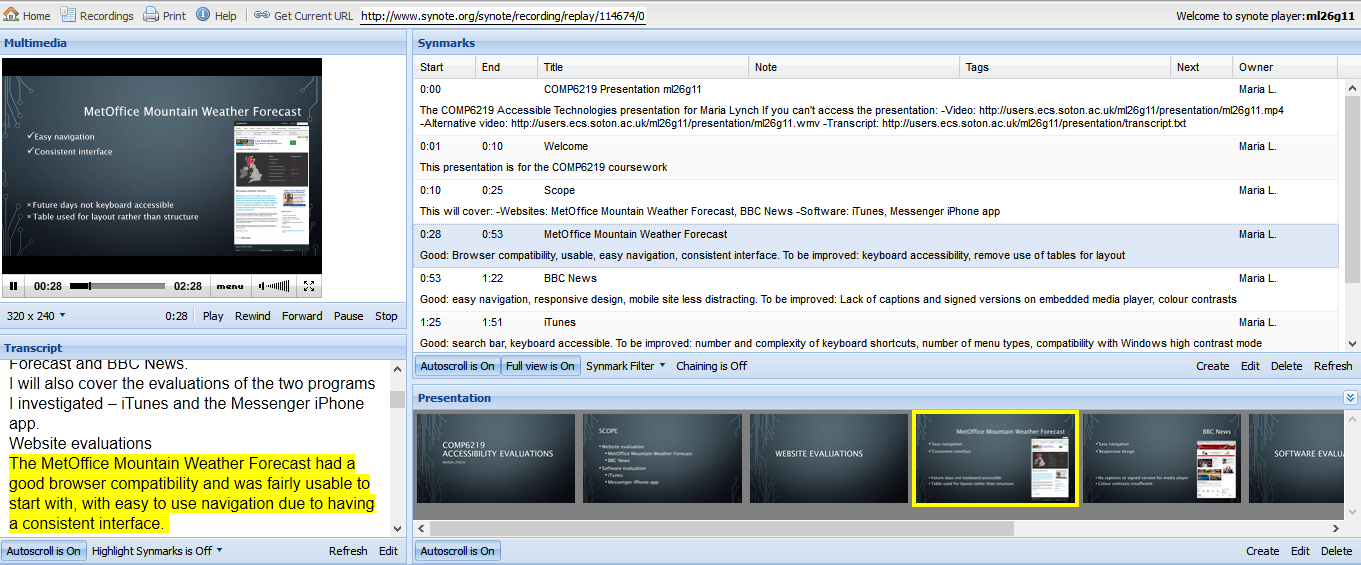
\includegraphics[scale=0.4]{../figures/synote_sync.png} 		
	\caption{\label{Figure:Synote} Screenshot of a Synote replay correctly synchronised (\url{http://www.synote.org/synote/recording/replay/114674/0} (Accessed: 15 Jan 15))}
\end{figure}

The textual element is a transcript of the video/audio. This aims to make the presentations more accessible for people with hearing impairments and cognitive difficulties. It also makes the presentation more easily searchable.

The bookmarks (known as Synmarks) can be used for many reasons. For example they could be used to provide summaries of the slides, make notes on the presentation or provide a direct copy of the text from the slides.

The images can be PowerPoint slides that are used in the presentation so that there can be other video to explain the slides at the same time.

Using the print function a screen reader friendly version of the presentation can be produced\footnote{\url{http://www.synote.org/synote/recording/handlePrint?id=114674&_part=&part=on&from=&to=&_synmarked=&_synmarked-user-1771=&_transcript=&transcript=on&_presentation=&presentation=on&slideHeight=&_synmarks=&synmarks=on&_synmarks-user-1771=&synmarks-user-1771=on&_synmarkId=&synmarkId=on&_synmarkTiming=&synmarkTiming=on&_synmarkTitle=&synmarkTitle=on&_synmarkNote=&synmarkNote=on&_synmarkTags=&synmarkTags=on&_synmarkOwner=&synmarkOwner=on&_synmarkNext=&synmarkNext=on}(Accessed: 15 Jan 15)}. This provides the transcripts, bookmarks and images in sequential order so that a screen reader can read all the text. This will be particularly useful to visually impaired users.

\section{Analytics}
\label{Section:Analytics}
Meaningful analysis of video data is difficult as you need to know the content of the video to understand why the sections may have been of interest to the user \citep{videoLectures}. \Citeauthor{videoLectures} \citep{videoLectures} proposes that extra features can be added to the video to aid automatic analysis to be useful, including: multiple (parallel) cognitive channels, semantic marking, transcripts and annotations. Video viewing styles have been researched for non-interactive videos (streaming) and in general four main styles were identified \citep{DeBoer}:
\begin{itemize}
\item \textbf{Linear} - A student watches a video in one-pass (uninterruptedly) from the beginning to the end
\item \textbf{Elaboration} - A student watches a video again after finishing the first time in one-pass
\item \textbf{Maintenance rehearsal} - A student watches parts of a video repeatedly
\item \textbf{Zapping} - A student skips through the instructional video at intervals of relatively short viewing times
\end{itemize}

With the growing popularity of \glspl{MOOC} analysis of video tutorials has been important to the educational industry to increase their usage. \Citeauthor{engagement} \citep{engagement} made several findings such as:
\begin{itemize}
\item Shorter videos are much more engaging
\item Khan-style tablet drawing tutorials are more engaging than PowerPoint slides or code screencast
\item Students engage differently with lecture and tutorial videos
\end{itemize}
These findings would also apply to video quizzes but as the quizzes add a new element to the material the interactions will be different and there will be many more things that could be learned from studying their usage patterns.

Currently there is little research into viewing styles of interactive videos with quizzes and polls in them as there are few tools to capture the necessary data. \Citeauthor{videoAnalytics} \citep{videoAnalytics} created an analytics tool that showed the quizzes separately to the video\footnote{\url{http://www.socialskip.org/home} (Accessed: 01 Dec 14)} to create graphs of video usage patterns. They used the YouTube player to collect the usage data and Google Drive to include quizzes. They chose to display this information in graphs of video time vs frequency.